\chapter{Implementation}
\label{ch:implementation}

\section{Decisions}
\subsection{OS}
The backend and model inference services run on \textbf{Linux}. It provides stable CUDA and PyTorch support for GPU acceleration, lowering resource consumption for long-running services, and better compatibility with our model stack (LLM, SigLIP, ComfyUI, FastAPI). Linux is also widely adopted in AI production environments, which aligns with our deployment needs.

\subsection{Programming Language}
\begin{itemize}
\item \textbf{Backend: }
The backend and AI modules are developed in \textbf{Python}. It offers mature AI tooling and integrates natively with our inference pipelines.
\item \textbf{frontend: }
The frontend will be built with \textbf{HTML}, \textbf{CSS}, and \textbf{JavaScript using Vue3}. It’s component-based and reactive architecture supports state management and real-time UI updates. This design allows new functions to be introduced by adding or extending components, without restructuring the overall page or application framework.
\end{itemize}

\subsection{Hardware}
This system relies on a \textbf{5090-level GPU} to support the generation of virtual try-on, embedded computing, and LLM inference. Its high memory capacity and throughput enable the model to run locally at a production speed, thereby avoiding cloud latency and token-related costs. This significantly enhances the user experience and ensures stable performance in future demonstrations and possible stress tests.

\subsection{Software}
\textbf{\large ComfyUI:}\\[0.4cm]
Initial attempts focused on local deployment of the Qwen-Image-Edit model. Due to network restrictions, offline installation became unreliable. We evaluated alternative methods and identified ComfyUI as a stable runtime environment that supports modular control, improving reproducibility and extensibility. Thus, We adopted a model demonstration architecture based on the ComfyUI platform, combined with a backend API invocation approach to implement the virtual try-on functionality.\\

\textbf{\large UniApp:}\\[0.4cm]
UniApp can compile a single codebase based on Vue3 into web pages, applications, and WeChat mini-programs. This ensures a unified development process and consistent user interface across different devices, facilitating future expansion of this project. The runtime adaptability also enables the same pages to be displayed on mobile phones, tablets, or browsers, thereby reducing maintenance work specific to certain platforms.


\subsection{Supporting Tools}
\begin{itemize}
\item \textbf{Figma} was used to design interactive UI prototypes and simulate user flows.
\item \textbf{DrawIO} was used to create high-level system architecture diagrams and module composition visuals.
\item \textbf{Visual Paradigm} was used to draw UML diagrams. 
\end{itemize}


\subsection{Virtual Try-on Model}
\label{Chapter: Model Comparison and Selection}

\textbf{\large Qwen-Image-Edit}\\[0.4cm]
Figures \ref{fig:qwen-comparison} and \ref{fig:qwen-comparison} demonstrate Qwen-Image’s editing performance. The model preserves the subject’s posture and background while generating new clothing with realistic material properties and shading, integrating it naturally into the original scene.

\begin{figure}[H]
  \centering
  \begin{minipage}{0.49\linewidth}
    \centering
    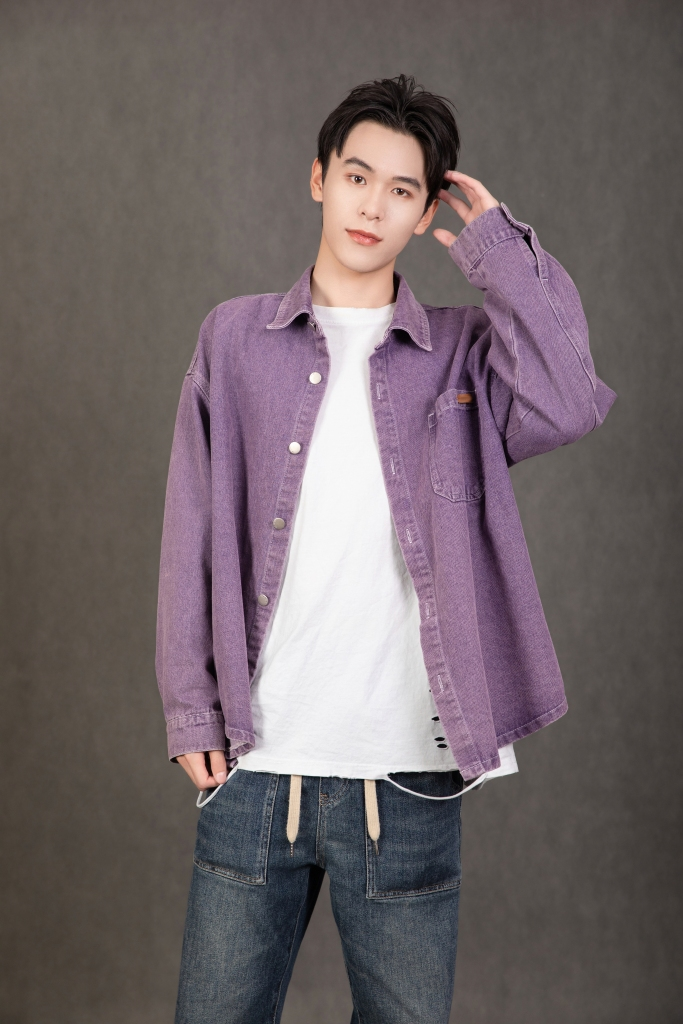
\includegraphics[width=\linewidth]{images/Section_6_Models/Qwen1.png}
    \caption{Original Body Image}
    \label{fig:qwen-comparison}
  \end{minipage}\hfill
  \begin{minipage}{0.49\linewidth}
    \centering
    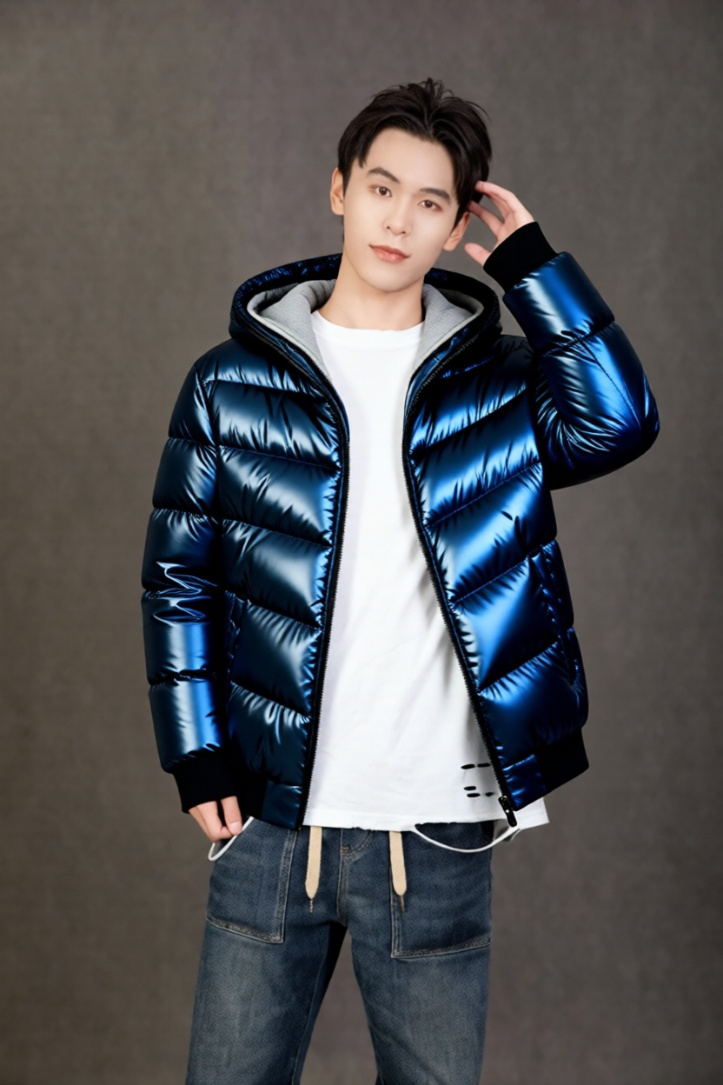
\includegraphics[width=\linewidth]{images/Section_6_Models/Qwen2.png}
    \caption{Qwen-Image-Edit Performance}
    \label{fig:qwen-additional}
  \end{minipage}
\end{figure}


\textbf{\large OOTDiffusion}\\[0.4cm]
Figures \ref{fig:ootd-comparison} and \ref{fig:ootd-additional} show OOTDiffusion’s performance. While the generated clothing is reasonably aligned with the body outline, the edited result shows noticeable deviations in arm posture and body proportions. In addition, subtle inconsistencies appear in local background regions, indicating that the model may alter non-target areas when handling complex clothing shapes or textures.

\begin{figure}[H]
  \centering
  \begin{minipage}{0.49\linewidth}
    \centering
    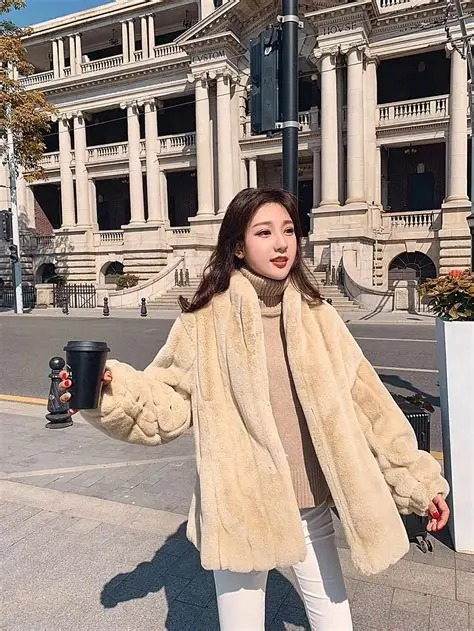
\includegraphics[width=\linewidth]{images/Section_6_Models/OOTD1.png}
    \caption{Original Body Image}
    \label{fig:ootd-comparison}
  \end{minipage}\hfill
  \begin{minipage}{0.49\linewidth}
    \centering
    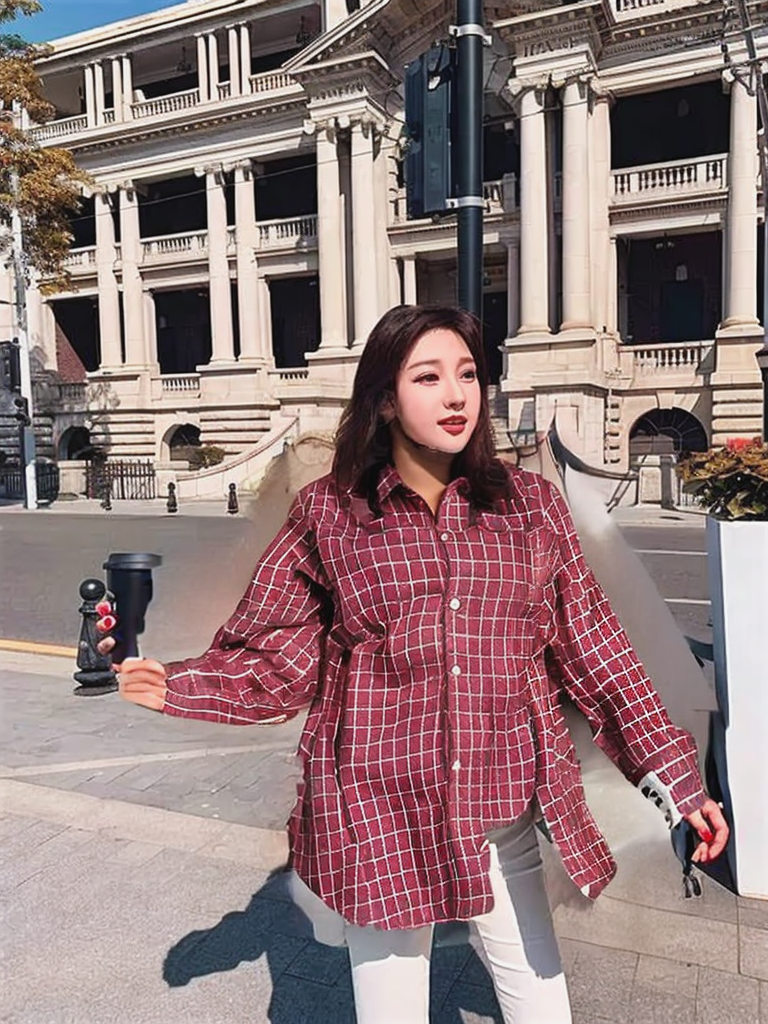
\includegraphics[width=\linewidth]{images/Section_6_Models/OOTD2.png}
    \caption{OOTD-Diffusion Performance}
    \label{fig:ootd-additional}
  \end{minipage}
\end{figure}


\textbf{\large Final Model Selection}\\[0.4cm]
OOTDiffusion often applies overly large masks during garment replacement, leading to background distortion and difficulty preserving fine-grained elements such as jewelry or small accessories. In contrast, Qwen-Image-Edit preserves posture, background, and local details, integrates uploaded clothing naturally, and can even adjust sleeve or pant lengths while plausibly completing exposed skin (more examples provided in Appendix \ref{appendix: Qwen}).

Thus, after conducting research and comparing the use of Qwen-Image-Edit and OOTD-diffusion, we determined that Qwen-Image-Edit would be the final model for our virtual try-on function.


\section{Results}
\subsection{Prototype}
This prototype implements all UI components defined in Chapter \ref{chapter_ui_design} (Initial UI Design) and integrates them into a complete workflow. Each page, including LLM Recommendation, Wardrobe Management, Wardrobe Analysis, and Virtual Try-On, corresponds to a core use case and provides seamless transitions across the user operation.
\begin{figure}[H]
    \centering
    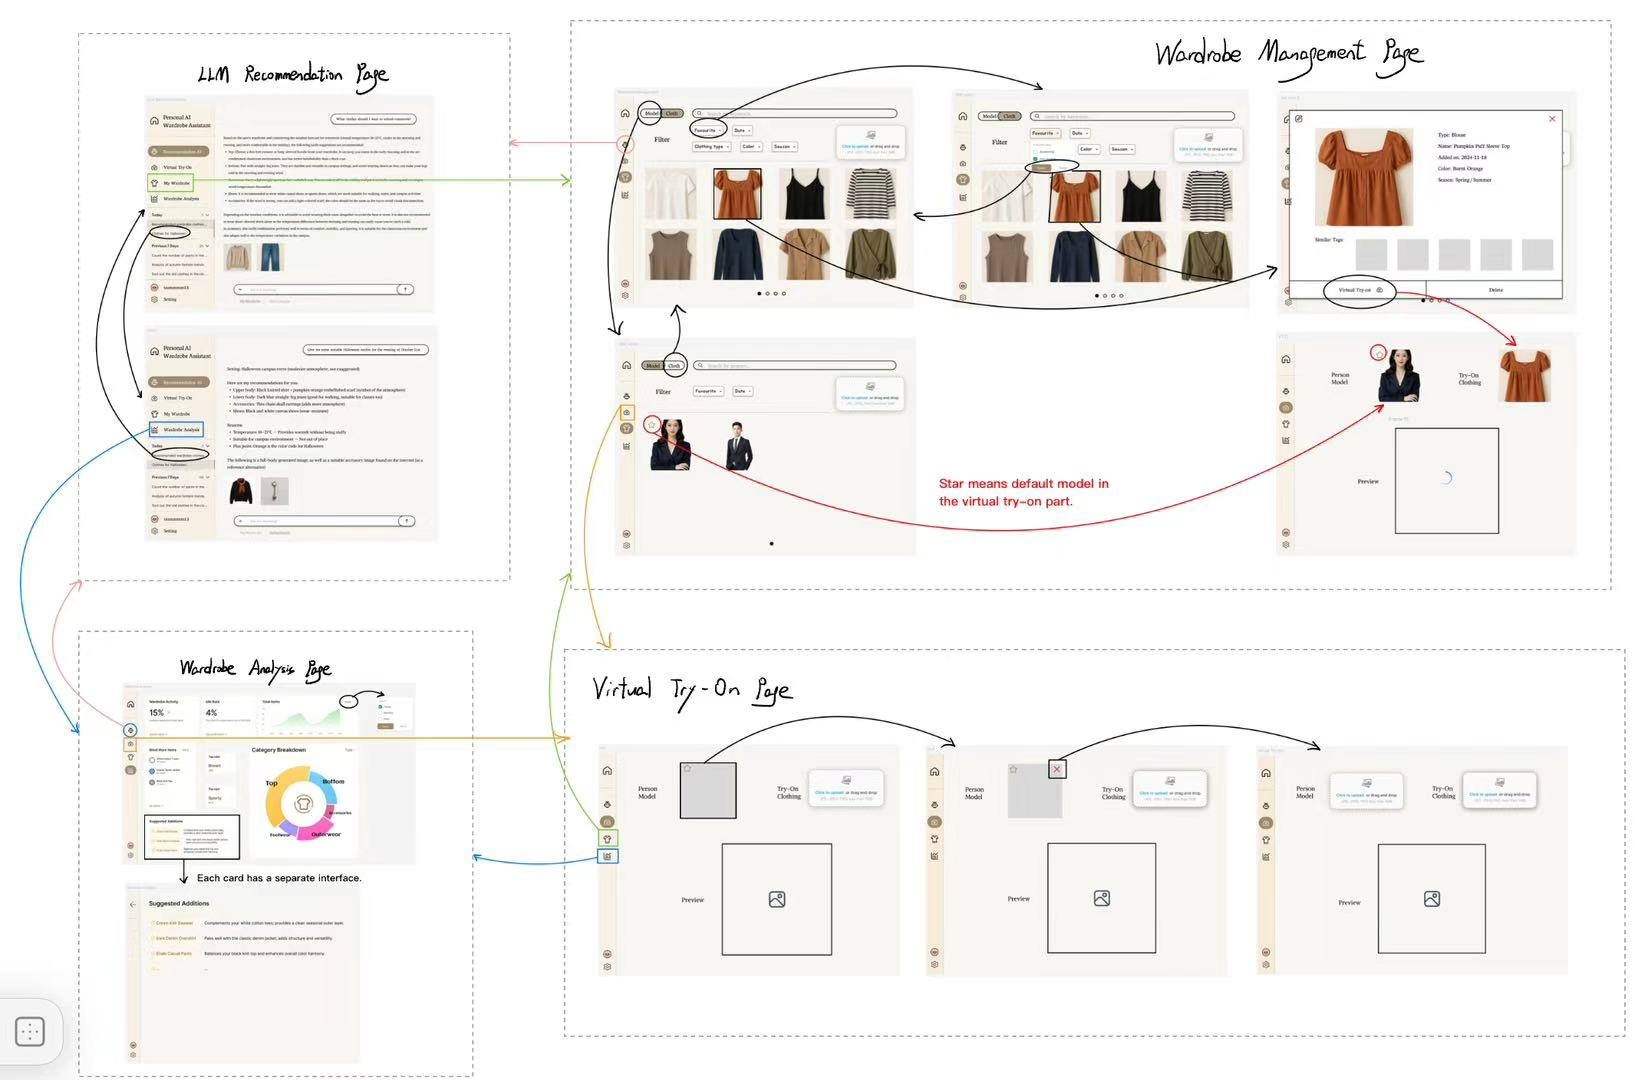
\includegraphics[width=1.5\textwidth, angle=270]{images/Section_6_Prototype/prototype.jpg}
    \caption{Prototype}
    \label{fig:Prototype}
\end{figure}


\subsection{Qwen-Image-Edit Model}
In this project, we decided to call the ComfyUI API to implement the virtual try-on functionality, and the implementation results are provided in Appendix \ref{appendix: Qwen}.

\textbf{\large ComfyUI Operation Procedure}

\begin{figure}[H]
    \centering
    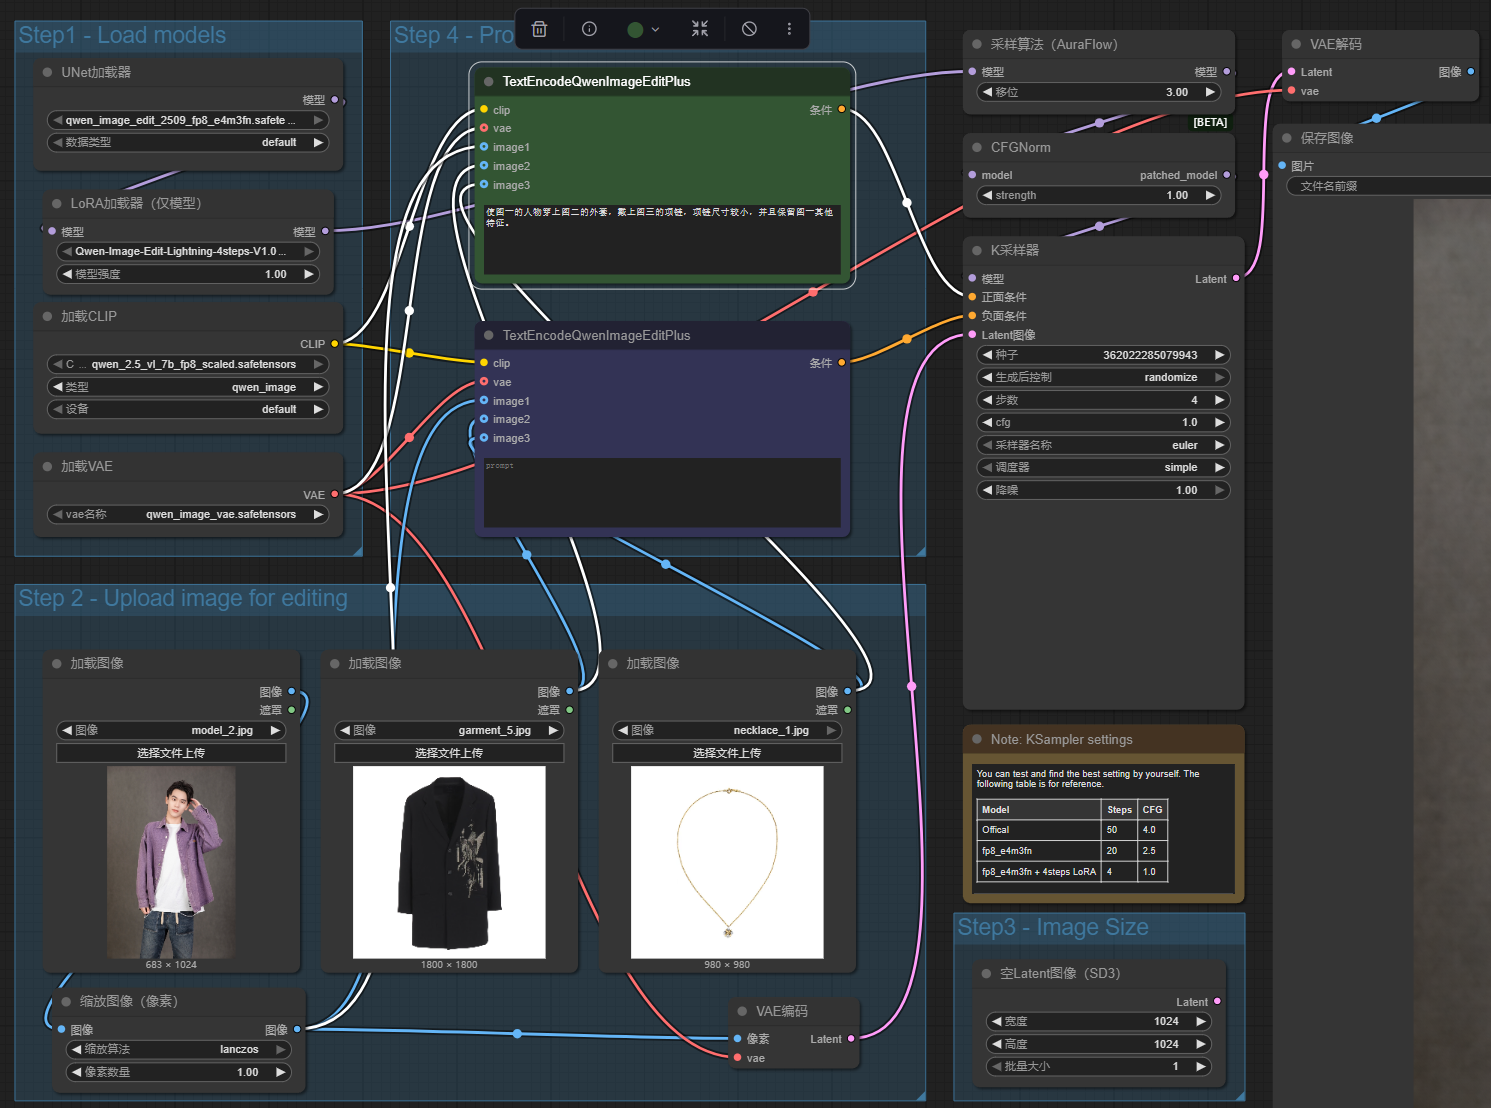
\includegraphics[width=0.95\textwidth]{images/Section_6.2.2/image.png}
    \caption{ComfyUI Workflow Interface for Qwen-Image-Edit}
    \label{fig:comfyui-detailed}
\end{figure}

\begin{enumerate}
    \item \textbf{Workflow Initialization}
    \begin{itemize}
        \item Open ComfyUI interface and load the pre-configured Qwen-Image-Edit workflow
        \item Ensure all necessary custom nodes are installed and updated
    \end{itemize}
    
    \item \textbf{Model Setup}
    \begin{itemize}
        \item Navigate to the model selection node and choose Qwen-Image-Edit
        \item Download necessary model components
        \item Check model compatibility and version requirements
    \end{itemize}
    
    \item \textbf{Input Configuration}
    \begin{itemize}
        \item In the image input nodes, upload:
        \begin{itemize}
            \item User reference photo (clear, full-body shot recommended)
            \item Clothing item image (front view, clean background)
            \item Accessory images if applicable (jewelry, shoes, etc.)
        \end{itemize}
        \item Adjust image preprocessing parameters if needed
    \end{itemize}
    
    \item \textbf{Generation Parameters}
    \begin{itemize}
        \item Set denoising strength (typically 0.7-0.9 for clothing try-on)
        \item Configure CFG scale for prompt adherence (recommended: 7.5-9.0)
        \item Adjust sampling steps for quality vs. speed balance
        \item Set random seed for reproducible results
    \end{itemize}
    
    \item \textbf{Execution and Monitoring}
    \begin{itemize}
        \item Click "Queue Prompt" to start generation
        \item Monitor progress in the execution queue
        \item Check console for any error messages or warnings
    \end{itemize}
    
    \item \textbf{Result Management}
    \begin{itemize}
        \item Review generated virtual try-on result
        \item Save output images
        \item Use API endpoints for automated batch processing
    \end{itemize}
\end{enumerate}
